\documentclass[11pt,a4paper]{article}
\usepackage[margin=23mm]{geometry}
\usepackage{amsmath,amssymb,graphicx,booktabs,longtable,array,float}
\usepackage{fontspec}
\setmainfont{lmroman10-regular.otf}[BoldFont=lmroman10-bold.otf,ItalicFont=lmroman10-italic.otf,BoldItalicFont=lmroman10-bolditalic.otf]
\setmonofont{lmmono10-regular.otf}
\usepackage{fvextra}
\usepackage[hidelinks]{hyperref}
\usepackage{microtype}
\setlength{\emergencystretch}{3em}
\setcounter{tocdepth}{1}
\begin{document}
\begin{titlepage}\centering
{\Large Lahore University of Management Sciences\par}\vspace{15mm}
{\huge AI651 -- Deep Learning for Space, Time and Graphs\par}\vspace{8mm}
{\Large Fall 2026, Assignment 3\par}\vspace{15mm}
{\LARGE Zain Gulbaz\par}\vspace{4mm}
{\Large Roll number: 25280005\par}\vspace{15mm}
{\large Repository: \texttt{GITHUB\_LINK\_HERE}\par}\vspace{8mm}
{\large CPU experiments, seed 42\par}\vfill
{\large 24 November 2026\par}
\end{titlepage}
\tableofcontents\newpage
\section{Q1 -- What does a sum remember?}
\subsection{(a) Affine messages}
Let $n_v=|\mathcal N(v)|$ and $S_v=\sum_{u\in\mathcal N(v)}x_u$. Then
\[
\sum_u\phi(x_u)=\sum_u(wx_u+c)=wS_v+cn_v.
\]
This also holds coordinatewise for vector parameters. Equal $(n_v,S_v)$ forces the same input to $\rho$ for every $w,c$, hence the same output for every $\rho$. The neighbourhoods $\{-1,+1,0\}$ and $\{0,0,0\}$ both have $(n_v,S_v)=(3,0)$ and aggregate $3c$, but have respectively one and three steady neighbours. No subsequent activation can recover information already discarded.
\subsection{(b) A scalar nonlinear encoding}
Set $B=K+1$, $\phi(-1)=1$, $\phi(0)=B$, $\phi(+1)=B^2$. If counts are $(a,b,c)$, the aggregate is $m=a+Bb+B^2c$. Each count is at most $K<B$, so no carries occur. Decode by $a=m\bmod B$, replace $m$ by $\lfloor m/B\rfloor$, recover $b=m\bmod B$, divide again, and obtain $c$. This is unique base-$B$ representation; it relies on exact arithmetic (large $K$ may require integers beyond floating-point precision). For counting only non-steady neighbours, $\phi(x)=x^2=|x|$ on this alphabet gives $a+c$ directly.
For K=8, the NumPy script checks all 164 triples with total size 1 through 8 (binomial(11,3)-1 = 164). Every code is unique and every decoded triple equals its input. The exact stdout and structured outputs are in logs/q1\_q2.log and results/q1\_q2.json.

\subsection{(c) Sum, mean and max of one-hot messages}
Write the aggregate as (z1,z2,z3) in slowing, steady, speeding-up order. The nine decisions below were checked against every multiset of size 1–8; exact rational keys avoid floating-point collisions for means.

\begin{table}[htbp]\centering\small\caption{All nine aggregation decisions. Task 1 counts steady; 2 tests slowing majority; 3 tests any slowing.}\begin{tabular}{llp{10cm}}\toprule
Task & Method & Decision and calculation\\\midrule
1 & sum & Yes: steady count = z2.\\
1 & mean & No: proportions lose size.\\
1 & max & No: presence loses multiplicity.\\
2 & sum & Yes: 2 z1 > z1+z2+z3.\\
2 & mean & Yes: z1 > 1/2.\\
2 & max & No: presence loses proportions.\\
3 & sum & Yes: z1 > 0.\\
3 & mean & Yes: z1 > 0.\\
3 & max & Yes: z1 = 1.\\
\bottomrule\end{tabular}\end{table}
Task 1, mean: neighbourhoods \{0\} and \{0, 0\} both give vector (0, 1, 0), but the required answers are 1 and 2. Both are nonempty and have at most eight members. Thus no function of the aggregate can distinguish them.

Task 1, max: neighbourhoods \{0\} and \{0, 0\} both give vector (0, 1, 0), but the required answers are 1 and 2. Both are nonempty and have at most eight members. Thus no function of the aggregate can distinguish them.

Task 2, max: neighbourhoods \{-1, +1, +1, +1, +1, +1, +1, +1\} and \{-1, -1, +1\} both give vector (1, 0, 1), but the required answers are False and True. Both are nonempty and have at most eight members. Thus no function of the aggregate can distinguish them.

\section{Q2 -- Which way is the slowdown moving?}
\subsection{(a) Symmetric spatial layer}
For the isolated spike, predictions at sensors $(19,20,21)$ are $(b,a,b)$ and targets are $(1,0,0)$. All other errors vanish, hence
\[
L(a,b)=(b-1)^2+a^2+b^2,\quad \partial_aL=2a=0,\quad \partial_bL=4b-2=0.
\]
Thus $a=0,b=1/2$, uniquely, since the Hessian is $\operatorname{diag}(2,4)$ and positive definite. The fitted readings are $(1/2,0,1/2)$ versus $(1,0,0)$, giving minimum squared error $1/2$. NumPy least squares confirms these coefficients.
\begin{figure}[htbp]\centering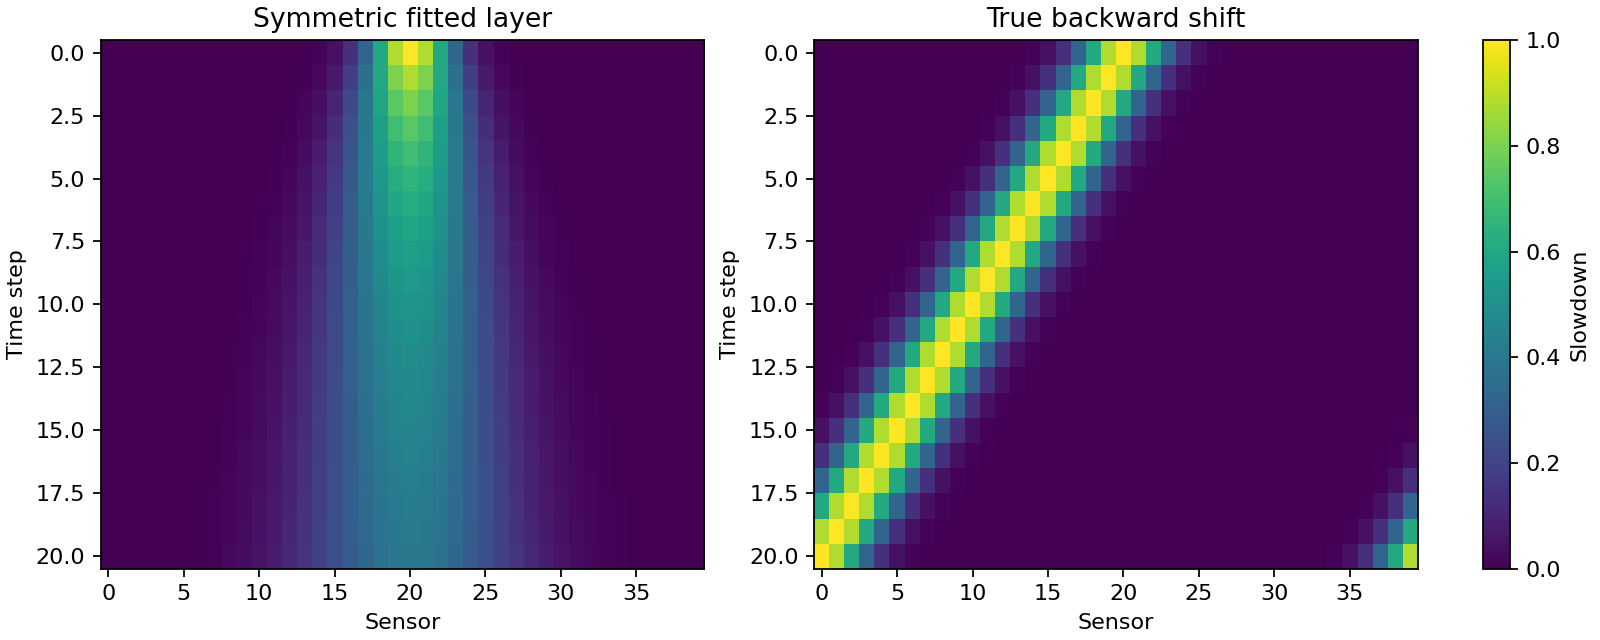
\includegraphics[width=.91\linewidth]{../figures/q2_rollout.png}\caption{Twenty recursive steps from the specified Gaussian bump, with a shared 0–1 colour scale and time rows 0–20.}\end{figure}
The fitted layer averages its two neighbours, producing symmetric diffusion: the bump broadens and its peak falls rather than translating against traffic. The true layer translates one sensor per step while preserving the profile and peak, including circular wraparound.

\subsection{(b) Directional neighbours}
Choose $a=0,w_-=0,w_+=1$. Substitution gives $\hat x_i(t+1)=x_{i+1}(t)$ identically for every snapshot. The cross-correlation kernel multiplying $[x_{i-1},x_i,x_{i+1}]$ is $[0,0,1]$; use circular padding of one sample on either side (a mathematical convolution convention reverses the stored kernel). Direction labels distinguish the ahead and behind neighbours, breaking the reflection ambiguity. Identical symmetric layers and pointwise nonlinearities alone preserve the isolated spike's reflection symmetry at sensors 19 and 21.
\subsection{(c) History with equal spatial weights}
Under backward motion, $x_{i-1}(t)=x_i(t-1)$. Therefore
\[
\hat x_i(t+1)=a x_i(t)+(b+c)x_{i-1}(t)+b x_{i+1}(t).
\]
For equality to $x_{i+1}(t)$ for every snapshot, equate coefficients: $a=0,b=1,c=-1$. The two spatial neighbours sum, and history subtracts the neighbour from which the current reading has already moved.
For forward motion $x_i(t)=x_{i-1}(t-1)$, so $x_i(t-1)=x_{i+1}(t)$ and the same coefficients yield
\[
\hat x_i(t+1)=x_{i-1}(t)+x_{i+1}(t)-x_{i+1}(t)=x_{i-1}(t).
\]
The same coefficients therefore \emph{also work for forward motion}; they do not fail for a consistent forward history. History breaks the snapshot reflection ambiguity by exposing the direction of travel across time; the subtraction adapts to whichever neighbour matches the previous local value. Constant or otherwise indistinguishable patterns can remain direction-ambiguous, but the required forecasts then agree.
\begin{table}[htbp]\centering\small\caption{Checks over a random 40-sensor ring; errors are floating-point roundoff.}\begin{tabular}{ll}\toprule
Numerical check (seed 42) & Max absolute error\\\midrule
Directional next snapshot & 0.000e+00\\
History, backward motion & 4.441e-16\\
History, forward motion & 2.220e-16\\
\bottomrule\end{tabular}\end{table}
\section{Q3 -- Dataset preparation and graph construction}\subsection{(a) Extraction, units and missingness}
The Kaggle CLI first listed all seven files. Only ca\_his\_raw\_2020.h5, ca\_his\_raw\_2021.h5, ca\_meta.csv and ca\_rn\_adj.npy were downloaded. The official San Diego notebook filters District == 11; here all 716 selected entries also have County == San Diego. Metadata ID strings select HDF columns, while the same rows’ ID2 values select both axes of the full graph. Assertions verify unique IDs, 716 sensors, column order and the ID2-to-ID mapping. The graph order convention comes from the official notebook; no raw graph ID labels are supplied independently.

PeMS Total Flow is the vehicle count across lanes during a five-minute interval, normalized upstream for good controller samples \cite{pems}. We therefore sum three counts, yielding vehicles per 15 minutes. The LargeST repository's CA preprocessing instead averages three values and rounds, retaining a five-minute-equivalent average volume \cite{repo}. Our sum preserves interval volume and follows the assignment's explicit interval-count instruction; metric magnitudes should not be compared directly with publications using the repository's averaging convention.

There are 7,636,666 nonfinite/missing raw SD readings out of the two-year complete grid (5.066183\%). Zeros are retained as valid readings, not reclassified as missing. Each year is reindexed to a complete five-minute grid, separately split at the prescribed boundaries, then causally forward-filled inside that split. Leading gaps in training use zero; leading gaps in validation/test use each sensor’s training-only mean after training imputation. No validation/test reading contributes to those fallback means or normalization. No backward fill or cross-boundary fill is used. Filling precedes summation so missing subintervals cannot silently shrink a quarter-hour count. Long outages can yield stale artificial plateaus; evaluation includes imputed targets and may understate error on genuinely observed traffic. PeMS may already impute upstream, and these files do not expose observation flags.

\begin{table}[htbp]\centering\small\caption{Chronological split sizes and missing raw 5-minute readings.}\begin{tabular}{lllll}\toprule
Split & 15-min steps & Windows & Raw missing & Missing \%\\\midrule
train & 35136 & 35125 & 3,095,400 & 4.101\\
val & 8640 & 8629 & 1,128,255 & 6.079\\
test & 26400 & 26389 & 3,413,011 & 6.019\\
\bottomrule\end{tabular}\end{table}
\begin{table}[htbp]\centering\small\caption{Distribution of per-sensor raw missingness, including complete outages.}\begin{tabular}{lllll}\toprule
Split & Min missing \% & Median missing \% & Max missing \% & All-missing sensors\\\midrule
train & 0.011 & 0.014 & 100.000 & 19\\
val & 0.046 & 0.046 & 100.000 & 43\\
test & 0.000 & 0.001 & 100.000 & 43\\
\bottomrule\end{tabular}\end{table}
There are 19 sensors with no finite raw readings throughout training and 43 throughout each of validation and test. For an entirely missing held-out sensor the chosen strategy supplies its training fallback mean at every step, not observed traffic. The primary required metrics include these synthetic constant targets and cannot establish real forecasting accuracy at those sensors. This is a material limitation when interpreting either the absolute errors or the benefit of spatial aggregation.

Per-sensor missing counts and percentages for each split are in results/missing\_per\_sensor.csv; Appendix A additionally reports each sensor’s combined two-year missing count and percentage. results/raw\_quality.csv separately records each year’s missing and zero counts.

\begin{figure}[htbp]\centering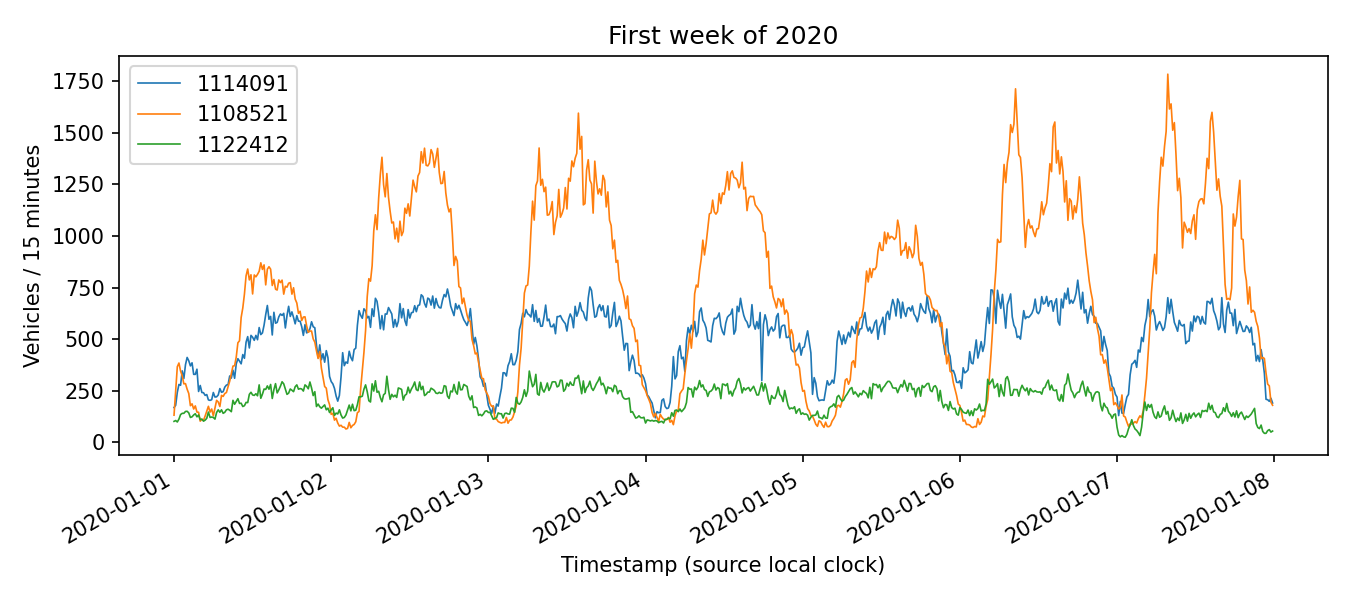
\includegraphics[width=.91\linewidth]{../figures/week_flow.png}\caption{One complete week of 15-minute interval vehicle counts at sensor indices 0, 357 and 715; selection was fixed before fitting.}\end{figure}
\subsection{(b) Road graph}
The graph has 716 nodes, 18,035 nonzero matrix entries including 716 diagonal entries, and 17,319 nonself directed edges. These are ordered matrix entries, not halved undirected counts. max |A-A\textasciicircum{}T| = 0.999999881, so the graph is directed. Nonself row degree has mean 24.189, minimum 0, and maximum 70.

The provided $A_{ij}$ is a thresholded Gaussian strength based on road driving distance, not a learned flow correlation. The LargeST paper describes querying driving distances only for candidates within a 4 km geodesic radius and pruning Gaussian strengths below 0.01 \cite{largest}. We preserve the supplied matrix. Operationally, row $i$ receives features from column $j$ through $(AZ)_i=\sum_j A_{ij}Z_j$. This aggregation convention is distinct from asserting a causal direction of traffic influence.
\begin{figure}[htbp]\centering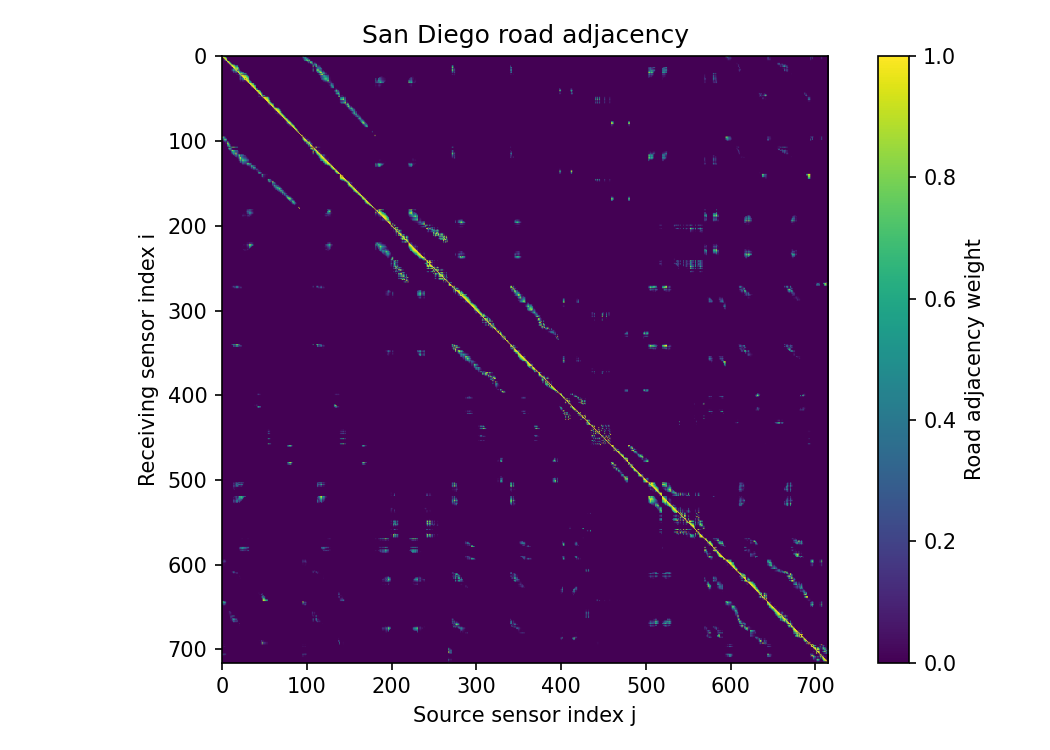
\includegraphics[width=.91\linewidth]{../figures/road_adjacency.png}\caption{Provided San Diego adjacency, ordered by the same metadata rows as the data tensor.}\end{figure}
\begin{figure}[htbp]\centering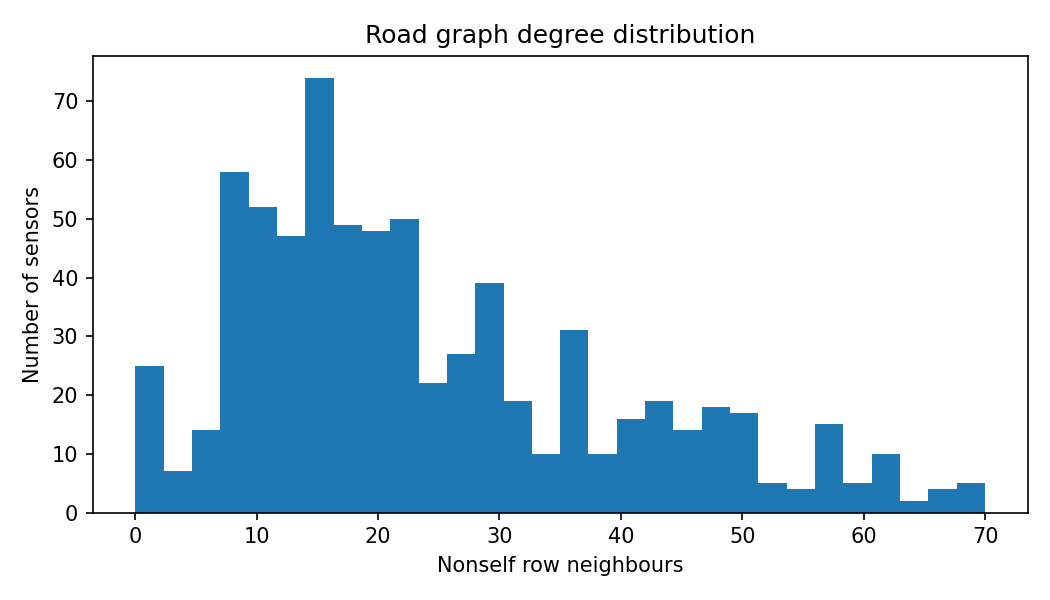
\includegraphics[width=.91\linewidth]{../figures/degrees.png}\caption{Number of nonzero nonself row neighbours for each of the 716 nodes.}\end{figure}
\subsection{(c) Neighbourhoods}
Selected sensor ID 1123003, tensor index 307, is the median-degree node (degree-based selection uses no traffic data). We exclude self-loops when listing neighbours. Its 20 one-hop sensor IDs are: 1108585, 1122487, 1113985, 1123002, 1108590, 1123029, 1123031, 1108592, 1120994, 1108489, 1122494, 1108429, 1123030, 1123006, 1108425, 1125201, 1125559, 1125527, 1125531, 1125546.

Its 38 distinct nonself sensors reachable through at most two row-neighbour steps (including one-hop nodes) are: 1108415, 1115749, 1108717, 1108585, 1122487, 1113985, 1123002, 1108590, 1123029, 1123031, 1108592, 1120994, 1121001, 1108597, 1121037, 1108595, 1108491, 1115838, 1108450, 1108489, 1122494, 1108429, 1123030, 1123006, 1108425, 1108519, 1121034, 1121035, 1125201, 1125559, 1125527, 1125610, 1125531, 1126292, 1125219, 1125546, 1113760, 1125575.

The provided matrix has a nonzero self-loop at the selected sensor. Under the assignment’s literal N(i) = \{j : Aij != 0\} definition, also include sensor 1123003 itself in each of the above sets (21 one-hop entries and 39 within-two-hop entries). The lists above isolate the 20 and 38 nonself spatial neighbours, respectively; the selected sensor is plotted separately.

Nearby road sensors can reveal arriving queues, shared commuting demand and upstream or downstream congestion before these appear fully at the target. One graph layer mixes direct neighbours; two stacked layers introduce neighbours of neighbours and multiply path weights. More layers may erase local differences through over-smoothing, propagate irrelevant or missing-data signals, and increase optimization difficulty. Directed reachability follows the supplied rows and is not symmetrized.

\begin{figure}[htbp]\centering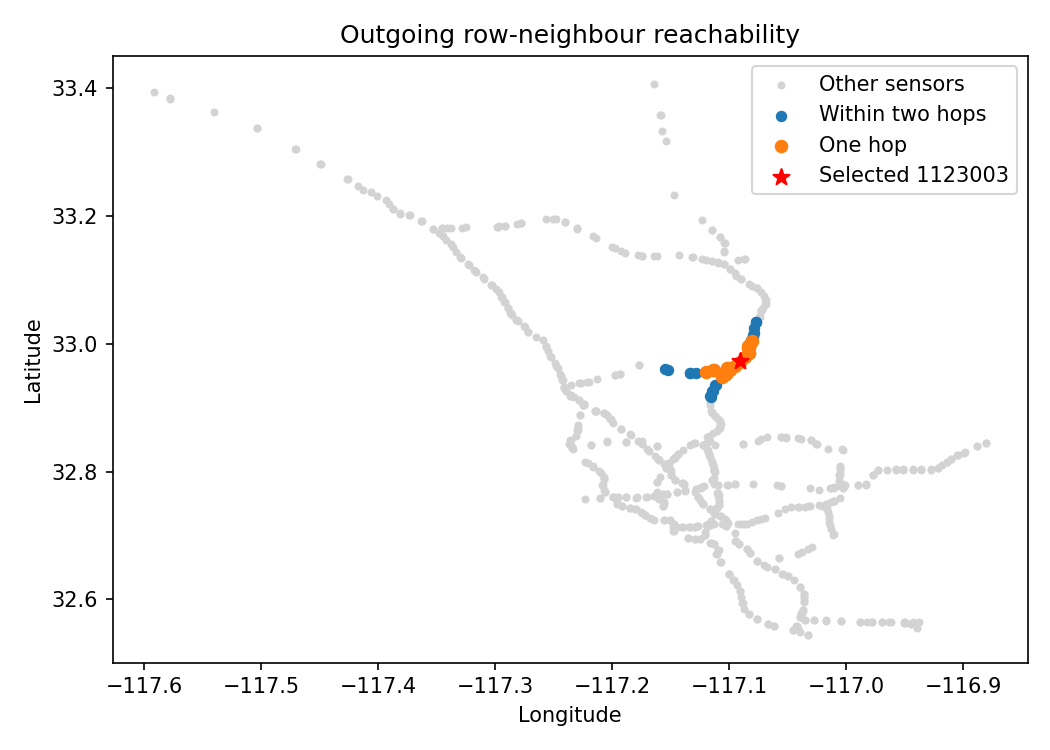
\includegraphics[width=.91\linewidth]{../figures/neighborhood.png}\caption{Selected sensor and its one-hop and within-two-hop sets on metadata latitude/longitude; grey points show all remaining sensors.}\end{figure}
\section{Q4 -- Forecasting architecture and protocol}\subsection{(a) Windows and leakage controls}
Every window has input shape (8,716,1) and target shape (4,716,1). Train uses all of 2020, validation January–March 2021, and test April–December 2021. Windows are constructed independently inside each array, with len(split)-11 samples; the first input starts at the split boundary and predicts steps 8–11. No input or target crosses a split. Training-only global mean is 584.440713411 and population standard deviation is 488.149905535 vehicles per 15 minutes. Both inputs and targets use these statistics. Graph embeddings learn only through training losses; validation selects the checkpoint, and the untouched common test period is used only for final evaluation and descriptive plots/analysis.

\subsection{(b) Architecture and training}
The shared temporal encoder applies two Conv1d layers per sensor: channels 1\ensuremath{\to}16\ensuremath{\to}16, kernel size 3, padding 1, ReLU after each. It retains the last temporal position, giving Z of shape (batch,716,16). All inputs are historical, so symmetric convolution padding within the eight-step history does not expose targets. The graph variants compute H = ReLU(A Z Wg), with one bias-free 16×16 graph projection. A shared linear 16\ensuremath{\to}4 head predicts four direct horizons. Every model adds the last normalized local reading to all four outputs as an identical persistence residual. Temporal-only feeds Z directly to the same head; the three STGNNs differ only in adjacency. Negative forecasts are not clipped.

All runs use CPU, seed 42 for Python/NumPy/PyTorch, Adam lr 0.001, batch size 64, shuffled full training windows, normalized MAE loss, patience 5 on full validation MAE, and the lowest-validation checkpoint. Hidden dimension 16 is within the assignment’s 16–32 CPU guidance. PyTorch deterministic algorithms are enabled, with no GPU operations or extra DataLoader workers. Each model has a fresh optimizer and a reset seed; shared encoder/head initialization matches. There is one graph layer, no dropout, and no weight decay. A complete one-epoch trial for each model precedes fresh final fits; trials are discarded and do not initialize final fits. The measured trials determine a common maximum of 30 epochs, capped at 30, reserving time inside a 7,200-second training budget. Per-epoch normalized train/validation MAE and times are recorded in JSON and logs.

\begin{table}[htbp]\centering\small\caption{Measured full-epoch timing tests and final model sizes/checkpoint selection.}\begin{tabular}{llllll}\toprule
Model & Trial train (s) & Trial incl. val (s) & Final epochs & Best epoch & Parameters\\\midrule
temporal & 15.526 & 17.536 & 18 & 13 & 916\\
fixed & 19.643 & 22.146 & 30 & 29 & 1172\\
adaptive & 21.908 & 24.614 & 30 & 29 & 15492\\
hybrid & 26.356 & 29.574 & 24 & 19 & 15493\\
\bottomrule\end{tabular}\end{table}
Training wall time includes epoch training, validation and in-memory best-state snapshots; final disk checkpoint writing, final val/test scoring, data loading and analysis are excluded. Timing-trial costs are reported separately. Different early-stopping epochs are allowed under the same rule; single-seed, time-limited results cannot establish statistical significance.

\subsection{(c) Temporal baseline comparison}
Temporal-only test MAE is 71.198; fixed-road STGNN test MAE is 69.308, a signed change of -1.890 vehicles per 15 minutes. The lowest measured test MAE belongs to adaptive (59.392). These results compare spatial aggregation with the same local temporal representation and persistence residual; they do not imply that graphs always help.

\section{Q5 -- Fixed, adaptive and hybrid graphs}\subsection{(a) Fixed}
Because $A$ is asymmetric we use $\widehat A_{ij}=(A+I)_{ij}/\sum_k(A+I)_{ik}$ rather than symmetric degree normalization. The original diagonal is retained and $I$ is added as specified, increasing self mass. All row sums equal one, including isolated nodes after adding identity. This tensor is a frozen buffer, not a trainable parameter. Nonzero $\widehat A_{ij}$ weights the feature of source $j$ in the update of receiver $i$.
\subsection{(b) Adaptive}
Learn $E_1,E_2\in\mathbb R^{716\times10}$, initialized from $\mathcal N(0,0.1^2)$, with $S=\operatorname{ReLU}(E_1E_2^\top)$. For CPU efficiency, retain the 20 largest scores per row \emph{before} normalization and apply softmax only to those scores:
\[
A^{\rm adp}_{ij}=\begin{cases}\exp(S_{ij})/\sum_{k\in T_i}\exp(S_{ik})&j\in T_i,\\0&\text{otherwise.}\end{cases}
\]
This is a sparsified version of row-softmax(ReLU($E_1E_2^\top$)); no road graph is used to select its support. Backpropagation flows through selected logits, softmax values and embeddings (and positive ReLU inputs), not through discrete top-k indices; excluded entries have zero direct gradient on that step, although their embeddings may change through other entries. There is no self-edge requirement. A sparse COO matrix multiplies node features while preserving value gradients. Nonnegative rows sum to one; the learned graph is generally directed.
\subsection{(c) Hybrid}
Both components are row-normalized. Let $\alpha=\operatorname{sigmoid}(\beta)$ with $\beta=0$ initially; then $A^{\rm hybrid}=\alpha\widehat A+(1-\alpha)A^{\rm adp}$, whose rows also sum to one. The scalar and embeddings receive gradients from training MAE. No extra sparsification follows mixing, so the support is the union of road and adaptive supports.
The selected hybrid checkpoint has alpha = 0.00255803. All models 2–4 share precisely the same temporal, graph-projection and forecast-head layers; graph construction is their only architectural difference. The results in Q6 include their measured error and training cost.

\begin{figure}[htbp]\centering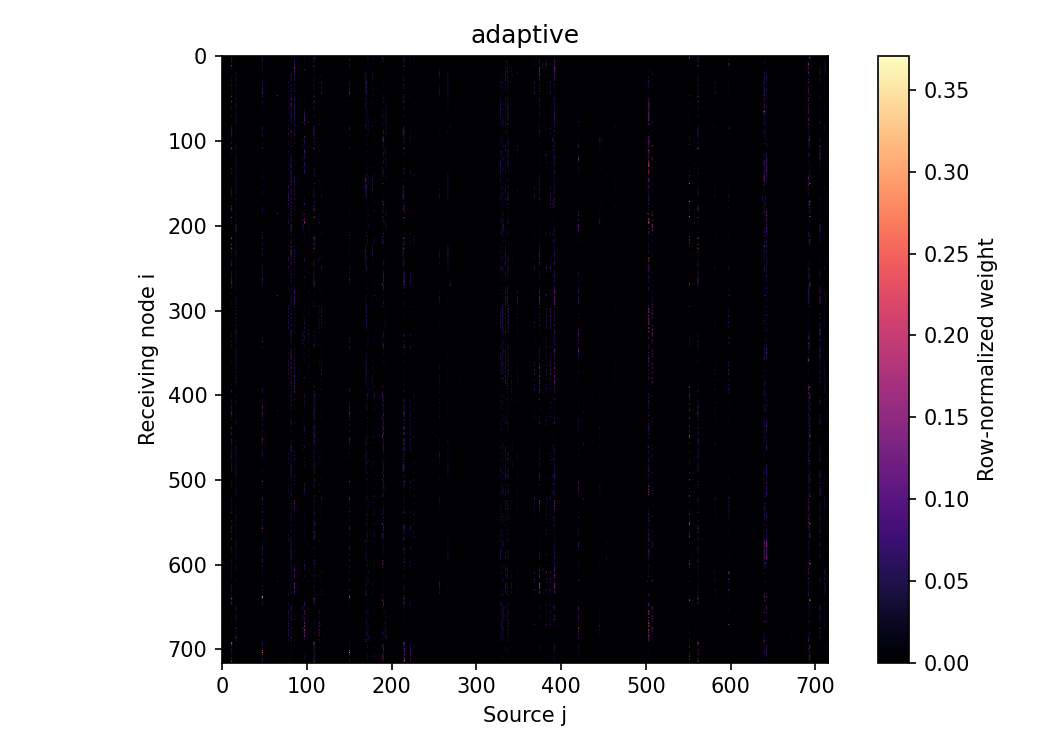
\includegraphics[width=.91\linewidth]{../figures/adaptive_adjacency.png}\caption{Learned standalone adaptive adjacency at its best-validation checkpoint; top-20 support per row.}\end{figure}
\begin{figure}[htbp]\centering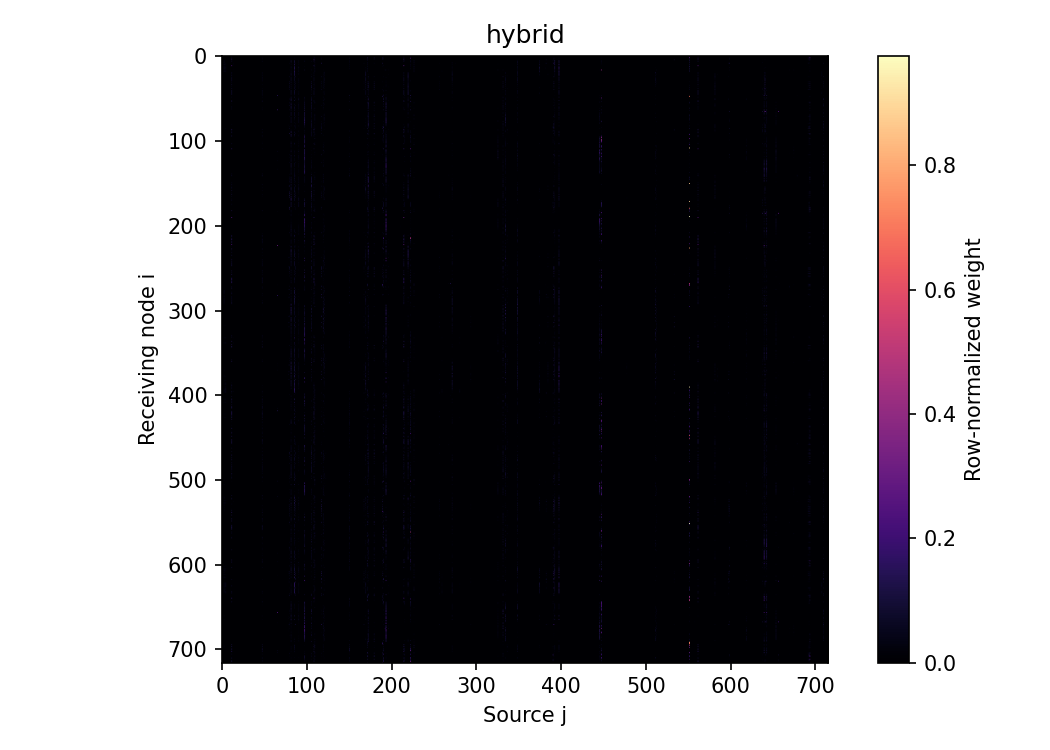
\includegraphics[width=.91\linewidth]{../figures/hybrid_adjacency.png}\caption{Hybrid adjacency at its best-validation checkpoint, including both fixed and learned components.}\end{figure}
\begin{figure}[htbp]\centering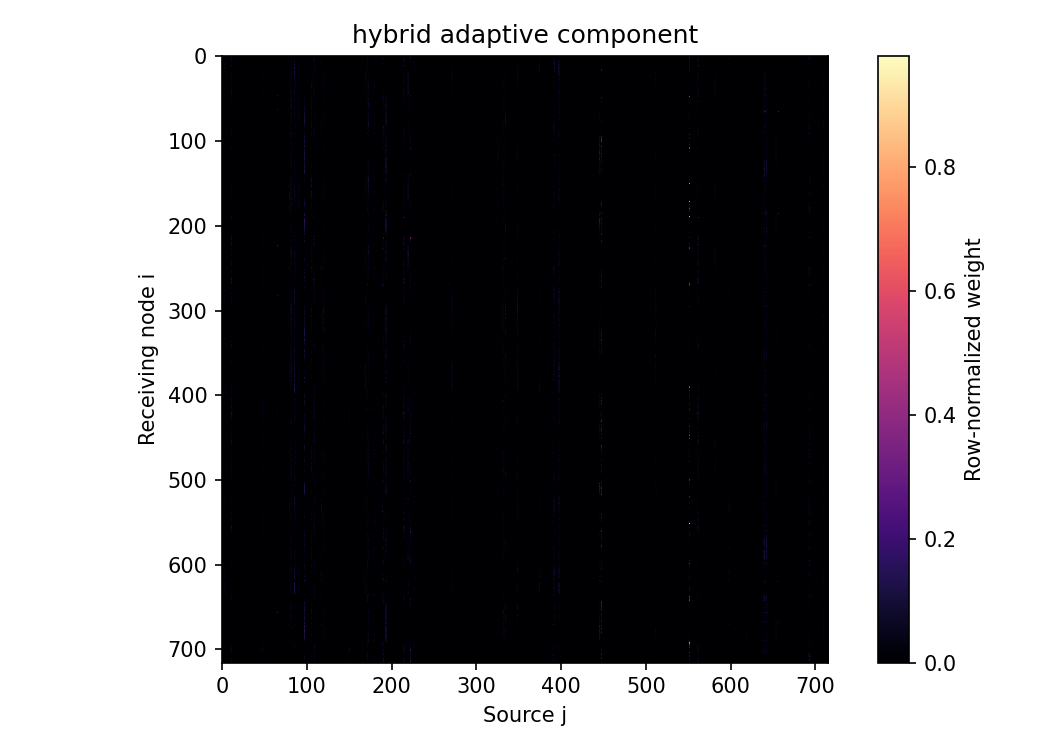
\includegraphics[width=.91\linewidth]{../figures/hybrid_adaptive_component_adjacency.png}\caption{Adaptive component inside the trained hybrid model; distinct from the standalone adaptive model.}\end{figure}
\section{Q6 -- Experimental analysis and interpretation}\subsection{(a) Forecasting comparison}
For errors e in original interval-count units, MAE = sum |e| / number of predictions and RMSE = sqrt(sum e\textsuperscript{2} / number of predictions). Overall metrics pool every test window, horizon and sensor, with each predicted entry equally weighted. Per-horizon metrics pool windows and sensors; overall RMSE is not an arithmetic mean of horizon RMSE. Overlapping targets therefore occur at different forecast origins, as intended. Validation metrics use the same definition on its own period.

\begin{table}[htbp]\centering\small\caption{Final comparison on the common April–December 2021 test period; errors in vehicles per 15 minutes.}\begin{tabular}{lllll}\toprule
Model & Adjacency & Test MAE & Test RMSE & Train time (s)\\\midrule
Temporal-only & None & 71.198 & 112.918 & 208.541\\
STGNN-Fixed & fixed & 69.308 & 109.646 & 593.163\\
STGNN-Adaptive & adaptive & 59.392 & 95.945 & 743.329\\
STGNN-Hybrid & hybrid & 59.946 & 97.013 & 678.964\\
\bottomrule\end{tabular}\end{table}
\begin{table}[htbp]\centering\small\caption{Validation totals and first two test horizons.}\begin{tabular}{lllll}\toprule
Model & Val MAE & Val RMSE & 15-min MAE/RMSE & 30-min MAE/RMSE\\\midrule
Temporal-only & 65.435 & 105.473 & 47.691 / 74.592 & 65.894 / 104.043\\
STGNN-Fixed & 63.184 & 101.813 & 47.016 / 73.400 & 64.200 / 101.290\\
STGNN-Adaptive & 52.905 & 87.455 & 43.782 / 69.469 & 57.125 / 92.050\\
STGNN-Hybrid & 53.841 & 89.152 & 44.521 / 70.740 & 57.831 / 93.457\\
\bottomrule\end{tabular}\end{table}
\begin{table}[htbp]\centering\small\caption{Remaining test horizons, in original units.}\begin{tabular}{lll}\toprule
Model & 45-min MAE/RMSE & 60-min MAE/RMSE\\\midrule
Temporal-only & 79.026 / 122.803 & 92.182 / 139.759\\
STGNN-Fixed & 76.741 / 119.189 & 89.275 / 135.041\\
STGNN-Adaptive & 65.472 / 104.777 & 71.188 / 112.001\\
STGNN-Hybrid & 65.824 / 105.817 & 71.608 / 112.740\\
\bottomrule\end{tabular}\end{table}
\begin{table}[htbp]\centering\small\caption{Validation horizons 15 and 30 minutes.}\begin{tabular}{lll}\toprule
Model & 15-min MAE/RMSE & 30-min MAE/RMSE\\\midrule
Temporal-only & 44.543 / 70.802 & 61.165 / 97.965\\
STGNN-Fixed & 43.647 / 69.333 & 59.010 / 94.746\\
STGNN-Adaptive & 40.241 / 64.973 & 51.743 / 85.000\\
STGNN-Hybrid & 41.191 / 66.703 & 53.039 / 87.356\\
\bottomrule\end{tabular}\end{table}
\begin{table}[htbp]\centering\small\caption{Validation horizons 45 and 60 minutes.}\begin{tabular}{lll}\toprule
Model & 45-min MAE/RMSE & 60-min MAE/RMSE\\\midrule
Temporal-only & 72.316 / 114.579 & 83.715 / 129.461\\
STGNN-Fixed & 69.687 / 110.626 & 80.390 / 124.264\\
STGNN-Adaptive & 58.221 / 95.805 & 61.415 / 99.841\\
STGNN-Hybrid & 58.924 / 97.406 & 62.209 / 101.113\\
\bottomrule\end{tabular}\end{table}
\begin{figure}[htbp]\centering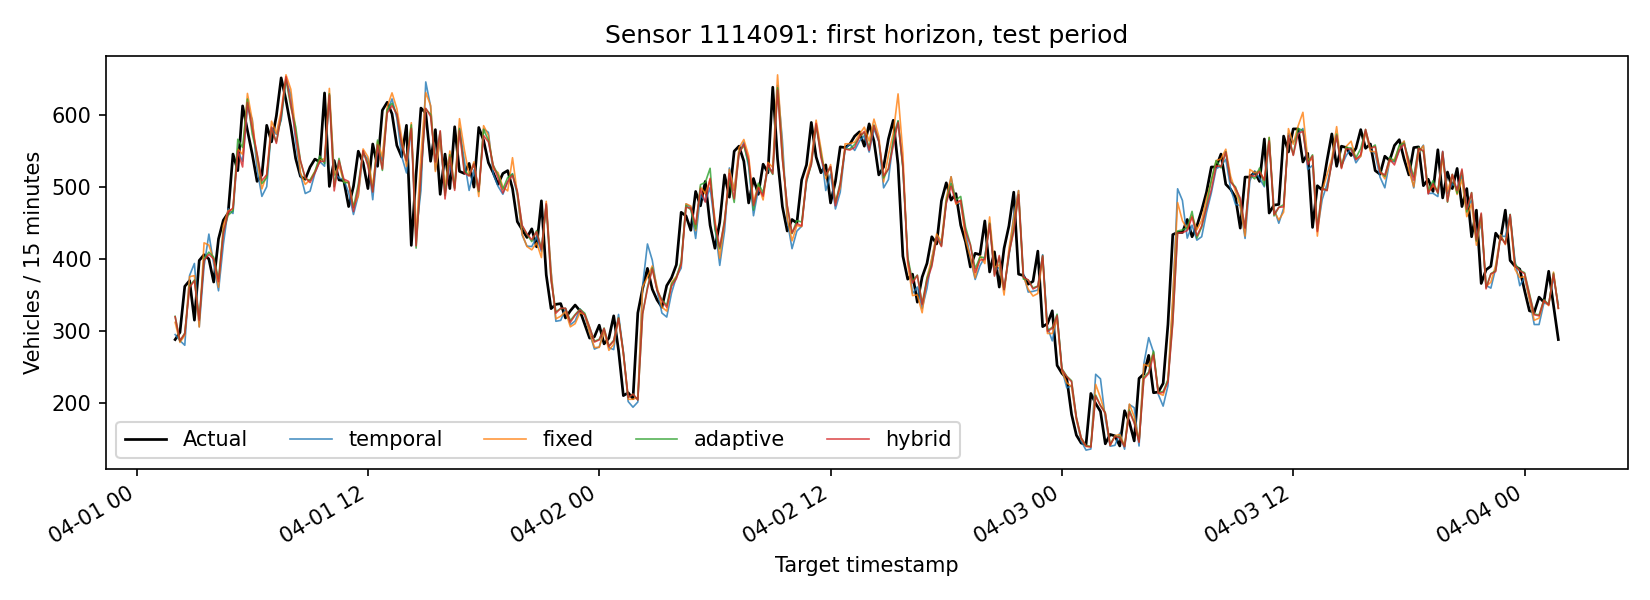
\includegraphics[width=.91\linewidth]{../figures/prediction_1114091.png}\caption{Actual and all four model predictions at sensor 1114091, first 288 test forecast origins, 15-minute horizon. Each prediction uses its own preceding eight true readings; this is rolling-origin forecasting, not a three-day recursive rollout.}\end{figure}
\begin{figure}[htbp]\centering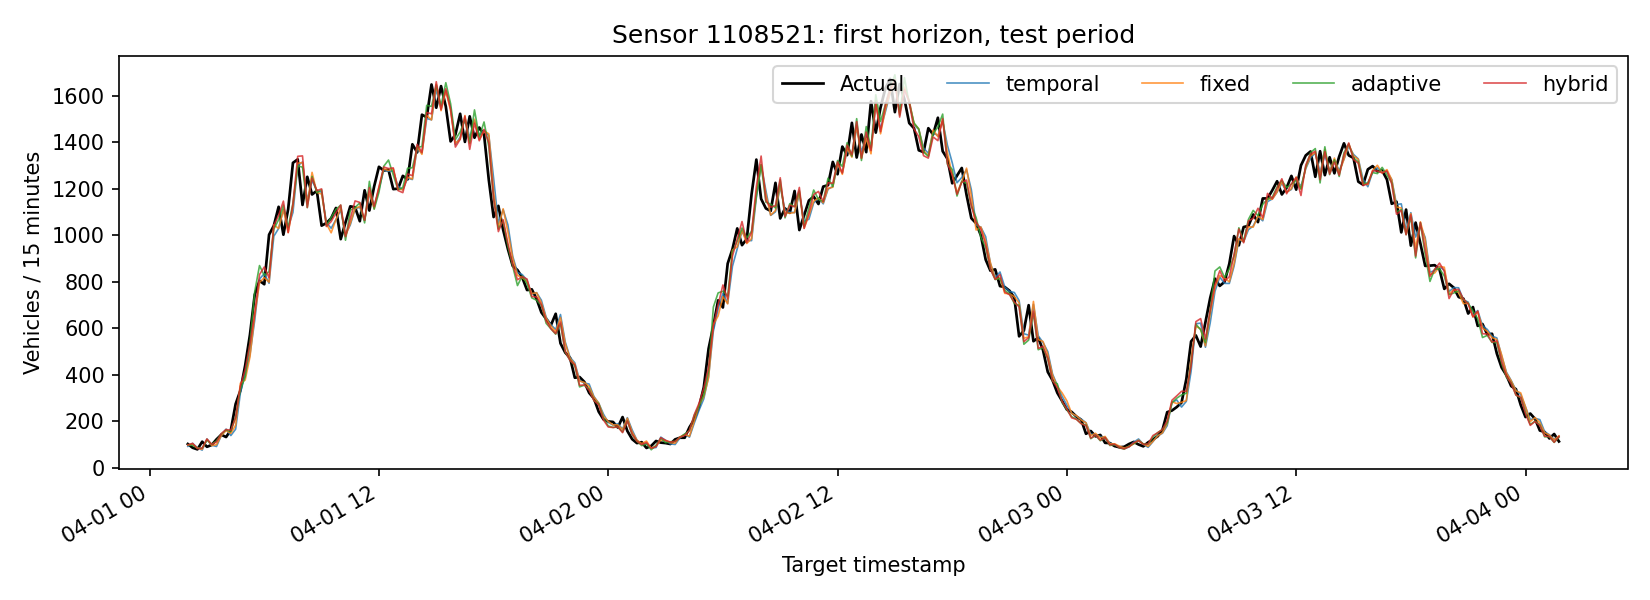
\includegraphics[width=.91\linewidth]{../figures/prediction_1108521.png}\caption{Actual and all four model predictions at sensor 1108521, first 288 test forecast origins, 15-minute horizon. Each prediction uses its own preceding eight true readings; this is rolling-origin forecasting, not a three-day recursive rollout.}\end{figure}
\begin{figure}[htbp]\centering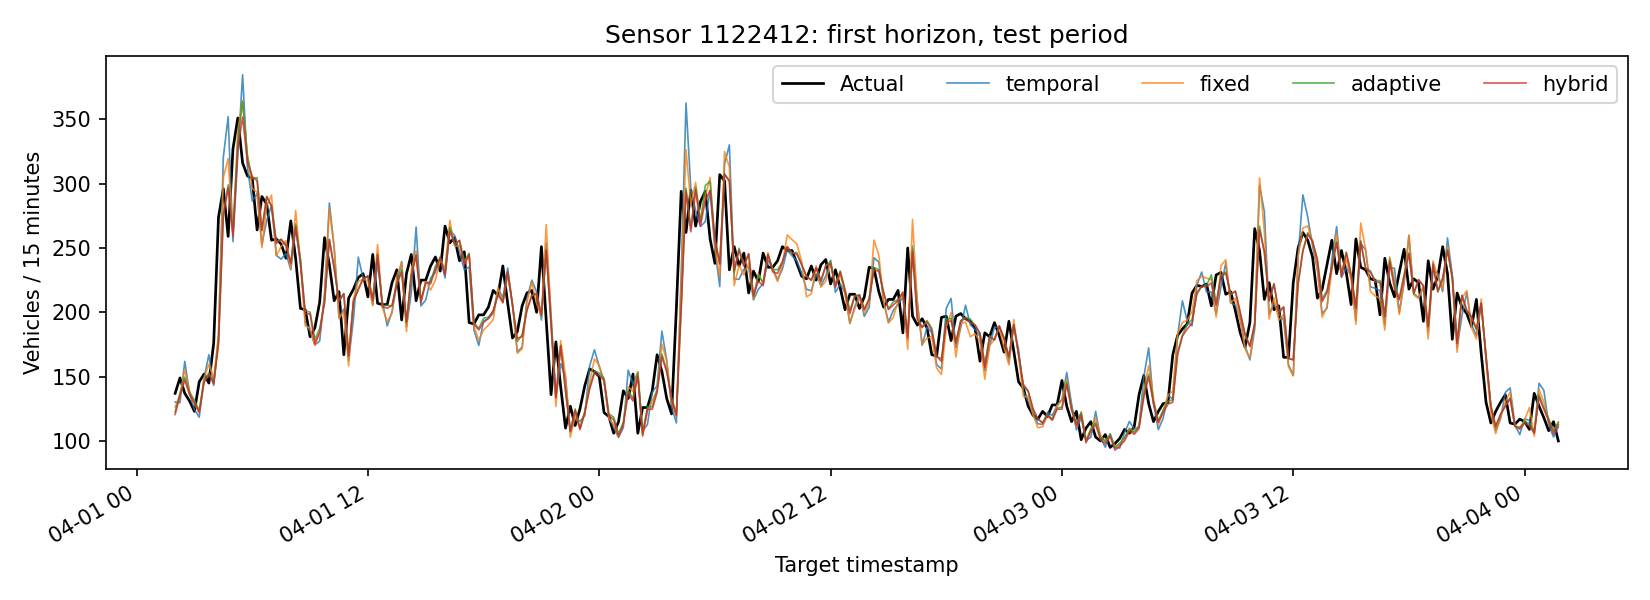
\includegraphics[width=.91\linewidth]{../figures/prediction_1122412.png}\caption{Actual and all four model predictions at sensor 1122412, first 288 test forecast origins, 15-minute horizon. Each prediction uses its own preceding eight true readings; this is rolling-origin forecasting, not a three-day recursive rollout.}\end{figure}
\begin{figure}[htbp]\centering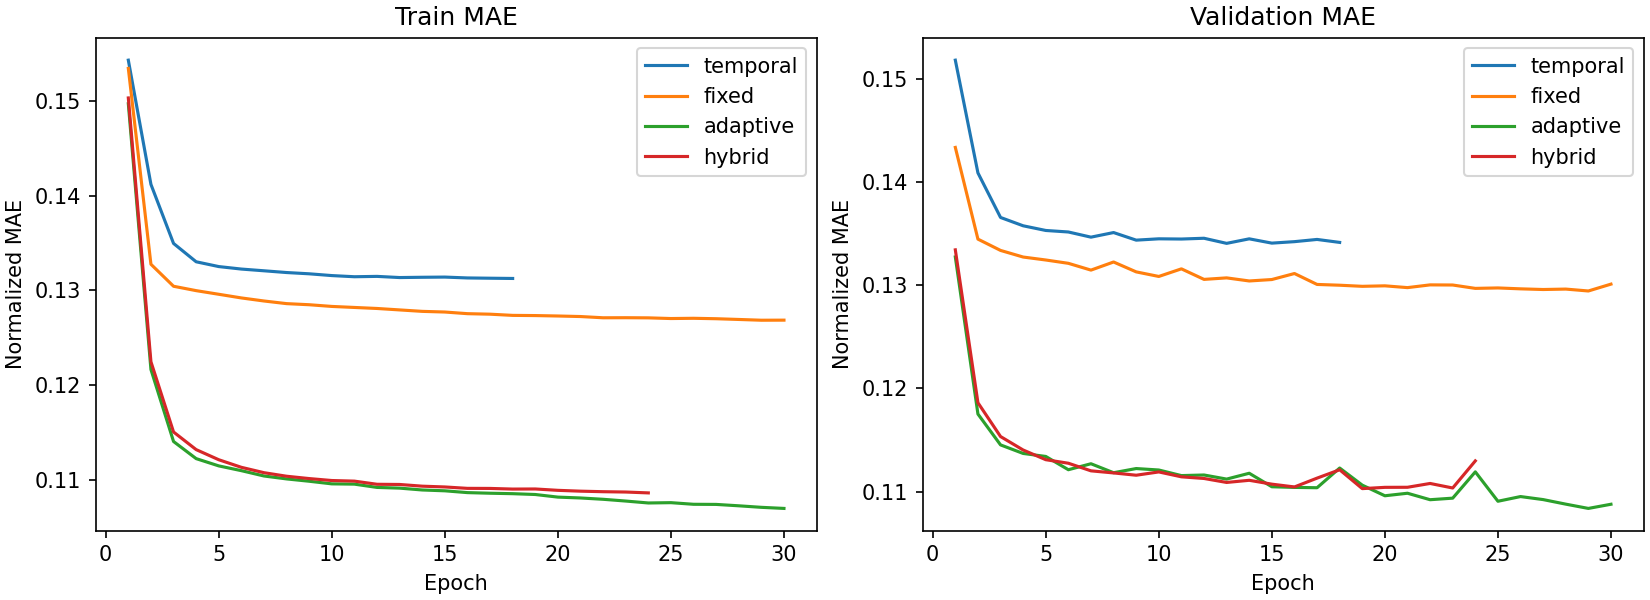
\includegraphics[width=.91\linewidth]{../figures/learning_curves.png}\caption{Full final-run training and validation normalized MAE histories; selected checkpoints minimize validation MAE.}\end{figure}
\subsection{(b) Graph structure analysis}
For each node, exclude its diagonal, rank learned weights, take its ten strongest neighbours and compute the fraction also present as nonzero nonself entries in the original road graph. Report the mean of these 716 fractions. Haversine distances use metadata coordinates with Earth radius 6,371 km. Road distances here are geodesic distances of directed nonzero road pairs, not the OSRM distances that generated the weights. The comparison uses 7,160 random ordered nonself pairs sampled with seed 42; they can repeat. Top-10 analysis uses the effective hybrid graph and separately its adaptive component, so physical mixing is not mistaken for discovered overlap.

\begin{table}[htbp]\centering\small\caption{Learned top-10 overlap and geographic-distance comparison. Road overlap excludes diagonal.}\begin{tabular}{p{4cm}rrrr}\toprule
Graph & Road overlap \% & Top-10 mean km & Road mean km & Random mean km\\\midrule
adaptive & 3.561 & 30.197 & 2.280 & 26.938\\
hybrid & 3.408 & 30.761 & 2.280 & 26.938\\
Hybrid adaptive part & 3.240 & 30.799 & 2.280 & 26.938\\
\bottomrule\end{tabular}\end{table}
\begin{figure}[htbp]\centering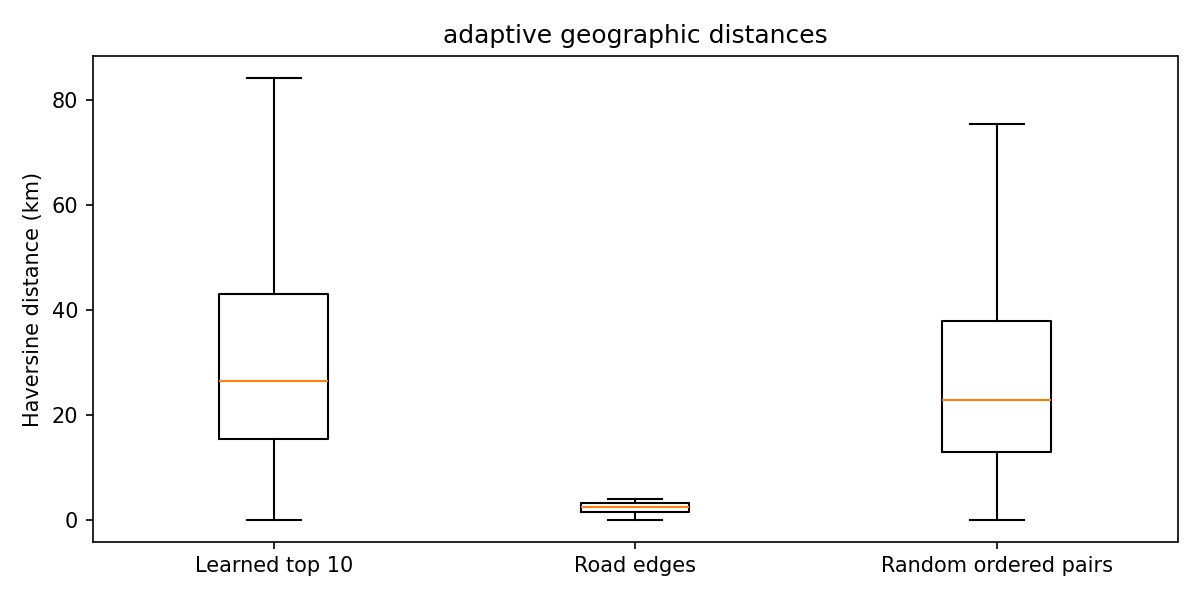
\includegraphics[width=.91\linewidth]{../figures/adaptive_distances.png}\caption{Adaptive top-10 nonself neighbour distances versus road neighbours and random pairs. Boxplots show medians and interquartile ranges; fliers are hidden.}\end{figure}
\begin{figure}[htbp]\centering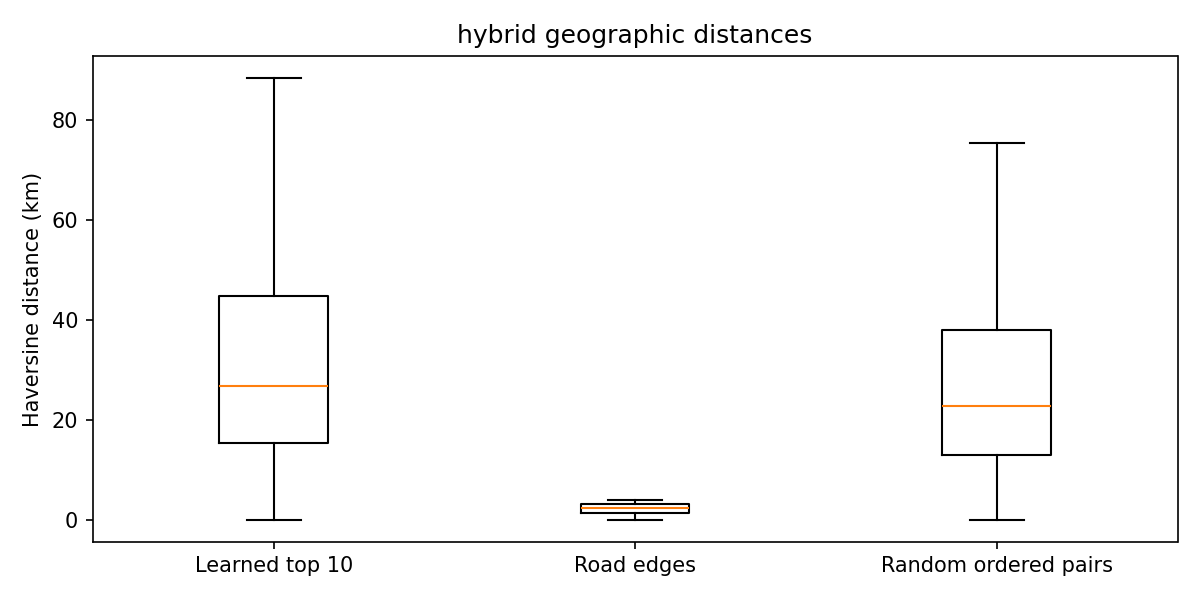
\includegraphics[width=.91\linewidth]{../figures/hybrid_distances.png}\caption{Hybrid top-10 nonself neighbour distances versus road neighbours and random pairs. Boxplots show medians and interquartile ranges; fliers are hidden.}\end{figure}
\begin{figure}[htbp]\centering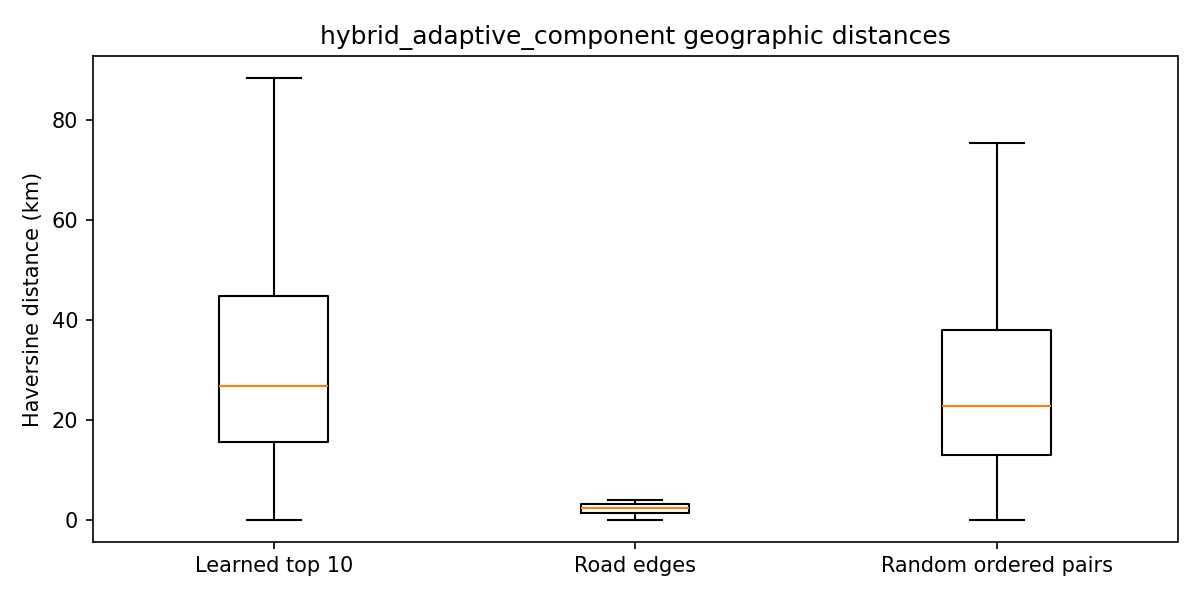
\includegraphics[width=.91\linewidth]{../figures/hybrid_adaptive_component_distances.png}\caption{Hybrid\_adaptive\_component top-10 nonself neighbour distances versus road neighbours and random pairs. Boxplots show medians and interquartile ranges; fliers are hidden.}\end{figure}
1. Strongest versus physical links: standalone adaptive overlap is 3.561\%; hybrid effective overlap is 3.408\%; the hybrid adaptive part is 3.240\%. The hybrid effective statistic partly reflects its built-in road component, not learned recovery of connectivity.

2. Geographic proximity: standalone adaptive top-10 links have mean 30.197 km and median 26.488 km, compared with road mean 2.280 km and random mean 26.938 km. Thus the observed learned distances must be judged against these distributions rather than assuming that learning recovers local roads.

The learned neighbours are not closer on average than the sampled random pairs, while the road edges provide the local-distance reference. This is descriptive evidence about this learned graph, not a significance test.

3. Dependencies absent from the physical graph: the following highest-weight positive standalone adaptive links have Aij=0 in the road matrix. They show that the parameterization represents nonlocal links, but do not prove causal influence or independently validate those dependencies. Shared daily demand, imputation patterns and finite-data overfitting can all create them.

\begin{table}[htbp]\centering\small\caption{Strong positive adaptive links absent from the road graph.}\begin{tabular}{llll}\toprule
Receiver ID & Source ID & Learned weight & Distance km\\\midrule
1122394 & 1116594 & 0.352353 & 28.804\\
1122380 & 1119653 & 0.348489 & 56.327\\
1125879 & 1123069 & 0.323991 & 25.207\\
1115348 & 1123069 & 0.321442 & 36.386\\
1111551 & 1123069 & 0.319146 & 16.741\\
\bottomrule\end{tabular}\end{table}
4. Why learning can help or hurt: fixed/adaptive/hybrid test MAEs are 69.308, 59.392, 59.946. Adaptive links can capture synchronized routes outside the road support, but embeddings add parameters, support selection is discrete, static averages miss changing congestion, and short single-seed fits may remain poorly optimized. Road aggregation can also dilute a useful local signal. The common persistence residual reduces the need for graph mixing. Training times in the comparison table quantify computational cost rather than assuming graph learning is free. The outcome supports the measured ranking for this protocol, not a general claim of superiority.

\subsection{(c) Critical discussion}
Lower forecast error does not establish actual road connectivity: optimizing prediction can exploit shared schedules or missing-data artifacts, and the measured standalone top-10 road overlap is only 3.561\%. Forecasting and physical graph recovery are different targets; no connectivity labels supervise the embeddings.

A hybrid may outperform either source by retaining local physical propagation while learning complementary global demand signals, with alpha regulating that tradeoff. Here alpha = 0.002558; its test MAE is 59.946 against fixed 69.308 and adaptive 59.392. The observed comparison, including any lack of improvement, is reported without claiming that mixing guarantees a gain.

Here the learned fixed-graph mixing mass is only 0.255803\%, so the selected hybrid is effectively adaptive. Its MAE exceeds standalone adaptive by 0.554; this run does not show a gain from combining the two sources.

A static graph averages morning/evening direction changes, weekday versus weekend demand, incidents, closures and evolving queues. A single scalar alpha cannot express such variation, and road-distance edges do not encode travel-time delays. A future time-conditioned graph could address this, but it would require leakage-safe training, stronger regularization and additional compute. The 2020-to-2021 split also faces pandemic-era demand shift; imputed targets and a single seed limit external validity.

\section{Q7 -- Reproducibility, hardware and limitations}
Hardware: Intel Xeon Gold 5218R at 2.10 GHz; 80 logical CPUs reported, 40 threads configured (at most half); approximately 376 GiB RAM from free -h. OS and exact CPU details are retained verbatim in results/hardware.txt. PyTorch 2.14.1+cpu, Python 3.10.12; CPU only, OMP\_NUM\_THREADS=40 and torch.set\_num\_threads(40), interop threads 1. All training is launched under nice -n 10; long setup/download/preprocessing/training/analysis jobs use nohup and per-job logs. No system packages, services or other applications are modified.

Measured total timing-trial cost is 93.870 seconds; final model training costs sum to 2223.998 seconds. Maximum epochs 30, hidden size 16 and top-k 20 were chosen for CPU feasibility. Training time includes validation, with the same timing boundaries for all variants. This is one seed with no uncertainty intervals, and early stopping can produce unequal amounts of optimization.

Environment deviation: the system Python 3.10 supports Kaggle 1.7.4.5, which fails with the new access-token format. A local Python 3.12 and .kaggle-venv run the latest Kaggle 2.2.5 (plus its missing six dependency), while .venv runs training. Both environments and their caches live in this folder; no credential contents were printed or copied. The report uses local Tectonic because no system TeX engine was available. No unrun metrics are included.

An initial Git status query inherited an ancestor repository and listed filenames outside the working folder. A dedicated local repository was initialized immediately; subsequent Git operations are scoped to this folder. No other application or service was changed.

\subsection{Exact reproduction sequence}
Run from the repository root. Install requirements in a local virtual environment; install CPU PyTorch from its CPU wheel index. If Python is below 3.11, reproduce the separate Kaggle environment using \texttt{scripts/setup.sh}. A configured Kaggle access token is required, but must never be committed. The commands below intentionally use nohup in the foreground: they survive a hangup and can also be launched in a persistent terminal.
\begin{Verbatim}[fontsize=\small,breaklines=true]
bash scripts/setup.sh
nohup bash scripts/download.sh > logs/download.log 2>&1 < /dev/null
OMP_NUM_THREADS=40 nohup .venv/bin/python -u scripts/preprocess.py > logs/preprocess.log 2>&1 < /dev/null
OMP_NUM_THREADS=40 .venv/bin/python q1_q2/verify.py
OMP_NUM_THREADS=40 .venv/bin/python -m scripts.check_models
OMP_NUM_THREADS=40 MKL_NUM_THREADS=40 OPENBLAS_NUM_THREADS=40 nohup nice -n 10 .venv/bin/python -u -m src.train > logs/training.log 2>&1 < /dev/null
OMP_NUM_THREADS=40 nohup .venv/bin/python -u -m scripts.analyze > logs/analysis.log 2>&1 < /dev/null
.venv/bin/python scripts/build_report.py
XDG_CACHE_HOME="$PWD/.cache" .tools/tectonic report/PA3_Zain_Gulbaz_25280005.tex
.venv/bin/python -m scripts.audit
\end{Verbatim}
src/train.py runs timing trials and all four experiments sequentially with the common protocol; results/config.json records the selected maximum and measured metadata. Checkpoints contain the best validation states. Processed SD arrays include IDs, graph indices, split timestamps and training statistics. results/results.json and results/results\_table.csv hold the final metrics. requirements.txt and requirements-kaggle.txt pin the actually installed packages. Raw and processed data, environments, checkpoints and logs are excluded from Git; the repository includes scripts, figures, summary CSV/JSON files and this report. The repository is initialized and committed locally; no remote is created and nothing is pushed.

\begin{thebibliography}{9}
\bibitem{largest} X. Liu et al. LargeST: A Benchmark Dataset for Large-Scale Traffic Forecasting. NeurIPS Datasets and Benchmarks, 2023. \url{https://arxiv.org/abs/2306.08259}.
\bibitem{repo} Official LargeST repository, San Diego extraction and CA processing notebooks. \url{https://github.com/liuxu77/LargeST}. Accessed 24 November 2026; downloaded notebook snapshots are in scripts/reference.
\bibitem{pems} Caltrans PeMS. Traffic data downloads, five-minute field specifications, Total Flow (vehicles / 5 min). \url{https://pems.dot.ca.gov/?dnode=pass}. Accessed 24 November 2026.
\bibitem{kaggle} LargeST dataset: \url{https://www.kaggle.com/datasets/liuxu77/largest}. CC BY-NC 4.0. Only required files downloaded; raw data are not redistributed in Git.
\end{thebibliography}
\clearpage\appendix\section{Per-sensor missingness}
Missingness below refers to the combined complete five-minute grids of 2020 and 2021, before any filling; the denominator is 210,528 readings per sensor. The machine-readable split-specific counts and percentages are in results/missing\_per\_sensor.csv. Zeros are not missing. Each row below packs three independent sensors to keep the appendix compact.
\small
\begin{longtable}{rrr|rrr|rrr}
\caption{Every sensor's raw missing count and percentage, two years combined.}\\
\toprule ID & Count & \% & ID & Count & \% & ID & Count & \%\\\midrule
\endfirsthead
\toprule ID & Count & \% & ID & Count & \% & ID & Count & \%\\\midrule\endhead
1114091 & 29 & 0.014 & 1118333 & 28 & 0.013 & 1118348 & 28 & 0.013\\
1114720 & 25 & 0.012 & 1118352 & 26 & 0.012 & 1118743 & 29 & 0.014\\
1120362 & 26 & 0.012 & 1118796 & 27 & 0.013 & 1118735 & 28 & 0.013\\
1118450 & 27 & 0.013 & 1114190 & 29 & 0.014 & 1118458 & 210528 & 100.000\\
1118479 & 31 & 0.015 & 1114205 & 28 & 0.013 & 1125469 & 30 & 0.014\\
1114211 & 28 & 0.013 & 1126864 & 28 & 0.013 & 1117762 & 28 & 0.013\\
1114219 & 28 & 0.013 & 1117782 & 28 & 0.013 & 1117809 & 28 & 0.013\\
1117748 & 708 & 0.336 & 1113976 & 28 & 0.013 & 1117741 & 26 & 0.012\\
1108603 & 26 & 0.012 & 1117835 & 25 & 0.012 & 1117717 & 25 & 0.012\\
1118078 & 27 & 0.013 & 1108611 & 27 & 0.013 & 1108613 & 26 & 0.012\\
1114050 & 27 & 0.013 & 1108617 & 28 & 0.013 & 1118496 & 29 & 0.014\\
1126411 & 28 & 0.013 & 1114805 & 30 & 0.014 & 1114035 & 28 & 0.013\\
1108547 & 25 & 0.012 & 1118707 & 28 & 0.013 & 1118521 & 27 & 0.013\\
1108665 & 28 & 0.013 & 1119637 & 29 & 0.014 & 1122594 & 27 & 0.013\\
1118537 & 27 & 0.013 & 1114296 & 28 & 0.013 & 1118544 & 27 & 0.013\\
1108719 & 30 & 0.014 & 1123086 & 131631 & 62.524 & 1123087 & 210528 & 100.000\\
1122536 & 30 & 0.014 & 1118170 & 27 & 0.013 & 1122552 & 28 & 0.013\\
1122575 & 28 & 0.013 & 1108437 & 25 & 0.012 & 1115277 & 26 & 0.012\\
1119828 & 28 & 0.013 & 1108507 & 30 & 0.014 & 1119679 & 25 & 0.012\\
1119850 & 28 & 0.013 & 1108509 & 29 & 0.014 & 1126614 & 30 & 0.014\\
1108512 & 28 & 0.013 & 1119659 & 28 & 0.013 & 1122507 & 28 & 0.013\\
1119865 & 131630 & 62.524 & 1125314 & 26 & 0.012 & 1119871 & 131628 & 62.523\\
1122512 & 30 & 0.014 & 1119879 & 27 & 0.013 & 1108651 & 27 & 0.013\\
1119890 & 28 & 0.013 & 1108663 & 26 & 0.012 & 1119903 & 25 & 0.012\\
1108682 & 26 & 0.012 & 1119921 & 28 & 0.013 & 1108687 & 28 & 0.013\\
1108659 & 26 & 0.012 & 1119928 & 25 & 0.012 & 1119934 & 29 & 0.014\\
1119941 & 27 & 0.013 & 1119947 & 28 & 0.013 & 1115289 & 37 & 0.018\\
1115304 & 27 & 0.013 & 1115306 & 28 & 0.013 & 1115314 & 27 & 0.013\\
1115323 & 25 & 0.012 & 1119960 & 28 & 0.013 & 1119972 & 27 & 0.013\\
1119984 & 27 & 0.013 & 1119990 & 28 & 0.013 & 1121692 & 27 & 0.013\\
1121707 & 25 & 0.012 & 1121715 & 29 & 0.014 & 1121724 & 26 & 0.012\\
1121731 & 30 & 0.014 & 1121737 & 28 & 0.013 & 1114228 & 28 & 0.013\\
1118326 & 27 & 0.013 & 1118341 & 28 & 0.013 & 1114721 & 26 & 0.012\\
1118365 & 26 & 0.012 & 1118372 & 30 & 0.014 & 1118379 & 28 & 0.013\\
1118695 & 29 & 0.014 & 1123133 & 29 & 0.014 & 1120356 & 28 & 0.013\\
1118413 & 27 & 0.013 & 1118428 & 28 & 0.013 & 1118472 & 29 & 0.014\\
1118442 & 210528 & 100.000 & 1122601 & 210528 & 100.000 & 1114240 & 29 & 0.014\\
1118465 & 26 & 0.012 & 1114254 & 27 & 0.013 & 1118076 & 27 & 0.013\\
1117755 & 27 & 0.013 & 1114268 & 28 & 0.013 & 1117774 & 29 & 0.014\\
1117789 & 29 & 0.014 & 1117810 & 28 & 0.013 & 1117683 & 39 & 0.019\\
1108417 & 26 & 0.012 & 1117734 & 29 & 0.014 & 1108605 & 26 & 0.012\\
1118702 & 27 & 0.013 & 1108609 & 27 & 0.013 & 1117871 & 25 & 0.012\\
1108615 & 27 & 0.013 & 1117818 & 29 & 0.014 & 1126426 & 39 & 0.019\\
1114806 & 29 & 0.014 & 1108711 & 27 & 0.013 & 1108693 & 28 & 0.013\\
1119307 & 27 & 0.013 & 1118529 & 29 & 0.014 & 1108667 & 28 & 0.013\\
1119817 & 26 & 0.012 & 1108669 & 26 & 0.012 & 1108452 & 26 & 0.012\\
1108498 & 27 & 0.013 & 1122544 & 30 & 0.014 & 1120754 & 28 & 0.013\\
1122567 & 28 & 0.013 & 1122560 & 27 & 0.013 & 1122583 & 29 & 0.014\\
1108434 & 26 & 0.012 & 1119834 & 26 & 0.012 & 1119528 & 30 & 0.014\\
1119842 & 30 & 0.014 & 1108468 & 28 & 0.013 & 1108471 & 28 & 0.013\\
1119653 & 210528 & 100.000 & 1108473 & 28 & 0.013 & 1119666 & 28 & 0.013\\
1108475 & 26 & 0.012 & 1108477 & 26 & 0.012 & 1108479 & 28 & 0.013\\
1119877 & 28 & 0.013 & 1108723 & 26 & 0.012 & 1119897 & 30 & 0.014\\
1108725 & 431 & 0.205 & 1119909 & 239 & 0.114 & 1108680 & 26 & 0.012\\
1119915 & 25 & 0.012 & 1108685 & 25 & 0.012 & 1108661 & 26 & 0.012\\
1108560 & 27 & 0.013 & 1108657 & 27 & 0.013 & 1108463 & 28 & 0.013\\
1108461 & 27 & 0.013 & 1108459 & 27 & 0.013 & 1108672 & 28 & 0.013\\
1115348 & 210528 & 100.000 & 1122257 & 30 & 0.014 & 1119954 & 26 & 0.012\\
1119966 & 26 & 0.012 & 1119978 & 28 & 0.013 & 1119997 & 26 & 0.012\\
1121702 & 26 & 0.012 & 1121712 & 27 & 0.013 & 1121722 & 210528 & 100.000\\
1121734 & 28 & 0.013 & 1111514 & 31 & 0.015 & 1108728 & 29 & 0.014\\
1114540 & 30 & 0.014 & 1113486 & 27 & 0.013 & 1115356 & 131631 & 62.524\\
1115413 & 27 & 0.013 & 1115432 & 29 & 0.014 & 1115438 & 29 & 0.014\\
1111551 & 210528 & 100.000 & 1115420 & 210528 & 100.000 & 1115426 & 28 & 0.013\\
1111566 & 29 & 0.014 & 1115444 & 27 & 0.013 & 1116783 & 27 & 0.013\\
1111565 & 27 & 0.013 & 1111549 & 30 & 0.014 & 1115450 & 27 & 0.013\\
1108366 & 28 & 0.013 & 1118752 & 30 & 0.014 & 1111564 & 29 & 0.014\\
1114573 & 27 & 0.013 & 1111535 & 29 & 0.014 & 1111534 & 28 & 0.013\\
1115463 & 1776 & 0.844 & 1111530 & 28 & 0.013 & 1111532 & 28 & 0.013\\
1111531 & 27 & 0.013 & 1122637 & 28 & 0.013 & 1122636 & 27 & 0.013\\
1122645 & 29 & 0.014 & 1122646 & 28 & 0.013 & 1115620 & 29 & 0.014\\
1115477 & 30 & 0.014 & 1116593 & 210528 & 100.000 & 1116594 & 210528 & 100.000\\
1115624 & 28 & 0.013 & 1115486 & 27 & 0.013 & 1115490 & 28 & 0.013\\
1115628 & 29 & 0.014 & 1114546 & 28 & 0.013 & 1116574 & 29 & 0.014\\
1115528 & 210528 & 100.000 & 1115517 & 131632 & 62.525 & 1115555 & 28 & 0.013\\
1115565 & 28 & 0.013 & 1111552 & 210528 & 100.000 & 1116165 & 42926 & 20.390\\
1115548 & 28 & 0.013 & 1111540 & 27 & 0.013 & 1115572 & 28 & 0.013\\
1111541 & 27 & 0.013 & 1115578 & 26 & 0.012 & 1111550 & 53 & 0.025\\
1122623 & 29 & 0.014 & 1115584 & 28 & 0.013 & 1115592 & 30 & 0.014\\
1115600 & 61 & 0.029 & 1127052 & 29 & 0.014 & 1118760 & 27 & 0.013\\
1108333 & 27 & 0.013 & 1127026 & 28 & 0.013 & 1118767 & 28 & 0.013\\
1108341 & 28 & 0.013 & 1108343 & 28 & 0.013 & 1108345 & 31 & 0.015\\
1108423 & 28 & 0.013 & 1108347 & 29 & 0.014 & 1115608 & 36 & 0.017\\
1108385 & 27 & 0.013 & 1108351 & 26 & 0.012 & 1108356 & 27 & 0.013\\
1111561 & 26 & 0.012 & 1108387 & 27 & 0.013 & 1108353 & 27 & 0.013\\
1111563 & 30 & 0.014 & 1108358 & 29 & 0.014 & 1115612 & 27 & 0.013\\
1115537 & 29 & 0.014 & 1115616 & 28 & 0.013 & 1115541 & 27 & 0.013\\
1111569 & 27 & 0.013 & 1108389 & 27 & 0.013 & 1108419 & 29 & 0.014\\
1111575 & 29 & 0.014 & 1113364 & 28 & 0.013 & 1108421 & 28 & 0.013\\
1126484 & 29 & 0.014 & 1126497 & 27 & 0.013 & 1126505 & 29 & 0.014\\
1126517 & 29 & 0.014 & 1119689 & 26 & 0.012 & 1119694 & 28 & 0.013\\
1119808 & 29 & 0.014 & 1118886 & 29 & 0.014 & 1123114 & 28 & 0.013\\
1118923 & 29 & 0.014 & 1108747 & 28 & 0.013 & 1108749 & 27 & 0.013\\
1108751 & 28 & 0.013 & 1119715 & 29 & 0.014 & 1117890 & 26 & 0.012\\
1108676 & 131628 & 62.523 & 1108528 & 27 & 0.013 & 1114044 & 26 & 0.012\\
1115649 & 27 & 0.013 & 1108655 & 27 & 0.013 & 1115656 & 27 & 0.013\\
1108531 & 28 & 0.013 & 1115663 & 25 & 0.012 & 1108534 & 24 & 0.011\\
1115672 & 25 & 0.012 & 1115713 & 26 & 0.012 & 1120611 & 345 & 0.164\\
1115721 & 28 & 0.013 & 1117909 & 27 & 0.013 & 1108536 & 40 & 0.019\\
1122469 & 30 & 0.014 & 1120167 & 32 & 0.015 & 1108439 & 31 & 0.015\\
1115739 & 42 & 0.020 & 1108415 & 26 & 0.012 & 1115749 & 31 & 0.015\\
1108717 & 24 & 0.011 & 1108585 & 27 & 0.013 & 1122487 & 26 & 0.012\\
1113985 & 27 & 0.013 & 1123003 & 79 & 0.038 & 1123002 & 28 & 0.013\\
1108590 & 27 & 0.013 & 1123029 & 26 & 0.012 & 1123031 & 29 & 0.014\\
1108592 & 27 & 0.013 & 1120994 & 26 & 0.012 & 1121001 & 28 & 0.013\\
1108597 & 25 & 0.012 & 1121037 & 30 & 0.014 & 1121038 & 28 & 0.013\\
1108595 & 25 & 0.012 & 1121105 & 30 & 0.014 & 1121099 & 31 & 0.015\\
1108562 & 29 & 0.014 & 1108767 & 29 & 0.014 & 1125872 & 30 & 0.014\\
1108769 & 28 & 0.013 & 1125886 & 27 & 0.013 & 1108771 & 30 & 0.014\\
1108773 & 28 & 0.013 & 1119736 & 29 & 0.014 & 1119743 & 30 & 0.014\\
1119749 & 27 & 0.013 & 1119762 & 27 & 0.013 & 1126812 & 28 & 0.013\\
1119774 & 26 & 0.012 & 1119780 & 29 & 0.014 & 1121751 & 28 & 0.013\\
1127045 & 29 & 0.014 & 1121757 & 28 & 0.013 & 1126722 & 27 & 0.013\\
1121763 & 29 & 0.014 & 1119683 & 28 & 0.013 & 1122942 & 29 & 0.014\\
1117920 & 29 & 0.014 & 1123165 & 27 & 0.013 & 1118900 & 26 & 0.012\\
1108753 & 28 & 0.013 & 1108755 & 28 & 0.013 & 1108757 & 30 & 0.014\\
1119707 & 30 & 0.014 & 1115763 & 27 & 0.013 & 1117931 & 30470 & 14.473\\
1108715 & 26 & 0.012 & 1115771 & 28 & 0.013 & 1108465 & 26 & 0.012\\
1115779 & 29 & 0.014 & 1108523 & 27 & 0.013 & 1115787 & 28 & 0.013\\
1108521 & 28 & 0.013 & 1115794 & 28 & 0.013 & 1115802 & 27 & 0.013\\
1115811 & 28 & 0.013 & 1117899 & 28 & 0.013 & 1108607 & 39 & 0.019\\
1115820 & 28 & 0.013 & 1122272 & 33 & 0.016 & 1108495 & 35 & 0.017\\
1122479 & 750 & 0.356 & 1108491 & 27 & 0.013 & 1115838 & 218 & 0.104\\
1108450 & 28 & 0.013 & 1108489 & 28 & 0.013 & 1122494 & 30 & 0.014\\
1108429 & 27 & 0.013 & 1123030 & 26 & 0.012 & 1123006 & 33 & 0.016\\
1108425 & 28 & 0.013 & 1108519 & 28 & 0.013 & 1108538 & 28 & 0.013\\
1121034 & 28 & 0.013 & 1121035 & 28 & 0.013 & 1121131 & 29 & 0.014\\
1121125 & 29 & 0.014 & 1108541 & 26 & 0.012 & 1121112 & 28 & 0.013\\
1121118 & 28 & 0.013 & 1108543 & 29 & 0.014 & 1121066 & 26 & 0.012\\
1108545 & 26 & 0.012 & 1125865 & 27 & 0.013 & 1108516 & 30 & 0.014\\
1125879 & 210528 & 100.000 & 1108558 & 27 & 0.013 & 1108556 & 28 & 0.013\\
1125265 & 30 & 0.014 & 1108554 & 28 & 0.013 & 1119756 & 30 & 0.014\\
1119768 & 29 & 0.014 & 1121748 & 28 & 0.013 & 1118557 & 28 & 0.013\\
1118567 & 27 & 0.013 & 1114141 & 29 & 0.014 & 1118575 & 30 & 0.014\\
1118636 & 27 & 0.013 & 1121774 & 30 & 0.014 & 1121794 & 27 & 0.013\\
1126575 & 28 & 0.013 & 1114520 & 29 & 0.014 & 1121806 & 30 & 0.014\\
1126770 & 29 & 0.014 & 1114529 & 29 & 0.014 & 1114511 & 28 & 0.013\\
1114162 & 30 & 0.014 & 1126257 & 28 & 0.013 & 1118552 & 28 & 0.013\\
1118562 & 28 & 0.013 & 1114166 & 28 & 0.013 & 1121771 & 28 & 0.013\\
1118591 & 28 & 0.013 & 1114177 & 131630 & 62.524 & 1118630 & 28 & 0.013\\
1126253 & 28 & 0.013 & 1121783 & 28 & 0.013 & 1126587 & 29 & 0.014\\
1121803 & 28 & 0.013 & 1126583 & 28 & 0.013 & 1121815 & 29 & 0.014\\
1111527 & 29 & 0.014 & 1111526 & 30 & 0.014 & 1114515 & 28 & 0.013\\
1108689 & 28 & 0.013 & 1108731 & 28 & 0.013 & 1108733 & 28 & 0.013\\
1108691 & 27 & 0.013 & 1108735 & 27 & 0.013 & 1108737 & 27 & 0.013\\
1125207 & 29 & 0.014 & 1125201 & 27 & 0.013 & 1125559 & 28 & 0.013\\
1125737 & 28 & 0.013 & 1125527 & 26 & 0.012 & 1108741 & 29 & 0.014\\
1125733 & 27 & 0.013 & 1108739 & 28 & 0.013 & 1125689 & 28 & 0.013\\
1113740 & 27 & 0.013 & 1125668 & 29 & 0.014 & 1125721 & 27 & 0.013\\
1125610 & 29 & 0.014 & 1125531 & 29 & 0.014 & 1126292 & 26 & 0.012\\
1125631 & 29 & 0.014 & 1125672 & 28 & 0.013 & 1125219 & 27 & 0.013\\
1125546 & 29 & 0.014 & 1113720 & 26 & 0.012 & 1113760 & 26 & 0.012\\
1125575 & 28 & 0.013 & 1108743 & 27 & 0.013 & 1113771 & 27 & 0.013\\
1112989 & 27 & 0.013 & 1119414 & 26 & 0.012 & 1108639 & 27 & 0.013\\
1116167 & 26 & 0.012 & 1108637 & 26 & 0.012 & 1108328 & 28 & 0.013\\
1115897 & 28 & 0.013 & 1108649 & 28 & 0.013 & 1108635 & 28 & 0.013\\
1108633 & 28 & 0.013 & 1108645 & 30 & 0.014 & 1108549 & 28 & 0.013\\
1116449 & 29 & 0.014 & 1108601 & 28 & 0.013 & 1108699 & 27 & 0.013\\
1108702 & 27 & 0.013 & 1115692 & 27 & 0.013 & 1108706 & 28 & 0.013\\
1126016 & 28 & 0.013 & 1126027 & 29 & 0.014 & 1112996 & 27 & 0.013\\
1108619 & 27 & 0.013 & 1108621 & 27 & 0.013 & 1116318 & 27 & 0.013\\
1108401 & 26 & 0.012 & 1108760 & 30 & 0.014 & 1108623 & 26 & 0.012\\
1108625 & 28 & 0.013 & 1118260 & 26 & 0.012 & 1108627 & 29 & 0.014\\
1108629 & 28 & 0.013 & 1108643 & 26 & 0.012 & 1108631 & 28 & 0.013\\
1116431 & 29 & 0.014 & 1108762 & 28 & 0.013 & 1108599 & 28 & 0.013\\
1108697 & 27 & 0.013 & 1108700 & 28 & 0.013 & 1108704 & 29 & 0.014\\
1126022 & 29 & 0.014 & 1126035 & 28 & 0.013 & 1108708 & 28 & 0.013\\
1113641 & 131630 & 62.524 & 1119449 & 27 & 0.013 & 1108380 & 26 & 0.012\\
1108378 & 27 & 0.013 & 1122956 & 27 & 0.013 & 1122951 & 27 & 0.013\\
1108376 & 28 & 0.013 & 1111568 & 28 & 0.013 & 1111559 & 27 & 0.013\\
1111567 & 28 & 0.013 & 1118648 & 27 & 0.013 & 1108374 & 26 & 0.012\\
1108505 & 27 & 0.013 & 1126373 & 28 & 0.013 & 1108503 & 28 & 0.013\\
1113966 & 25 & 0.012 & 1108501 & 27 & 0.013 & 1113181 & 30 & 0.014\\
1118989 & 131628 & 62.523 & 1111558 & 29 & 0.014 & 1108285 & 27 & 0.013\\
1108287 & 26 & 0.012 & 1108289 & 28 & 0.013 & 1108291 & 28 & 0.013\\
1108293 & 27 & 0.013 & 1108295 & 28 & 0.013 & 1108297 & 28 & 0.013\\
1108302 & 26 & 0.012 & 1108304 & 25 & 0.012 & 1108306 & 26 & 0.012\\
1108308 & 26 & 0.012 & 1108311 & 26 & 0.012 & 1108313 & 25 & 0.012\\
1108315 & 27 & 0.013 & 1108317 & 27 & 0.013 & 1113173 & 28 & 0.013\\
1113126 & 26 & 0.012 & 1120121 & 26 & 0.012 & 1112964 & 30 & 0.014\\
1113267 & 28 & 0.013 & 1113266 & 29 & 0.014 & 1113147 & 29 & 0.014\\
1113292 & 29 & 0.014 & 1113297 & 27 & 0.013 & 1113017 & 26 & 0.012\\
1113159 & 29 & 0.014 & 1113301 & 31 & 0.015 & 1113308 & 30 & 0.014\\
1113187 & 28 & 0.013 & 1108372 & 27 & 0.013 & 1108299 & 210528 & 100.000\\
1111555 & 29 & 0.014 & 1111557 & 29 & 0.014 & 1113915 & 28 & 0.013\\
1113222 & 29 & 0.014 & 1113894 & 27 & 0.013 & 1113327 & 27 & 0.013\\
1113413 & 28 & 0.013 & 1114006 & 31 & 0.015 & 1114018 & 29 & 0.014\\
1108323 & 210528 & 100.000 & 1113138 & 27 & 0.013 & 1108326 & 26 & 0.012\\
1111554 & 27 & 0.013 & 1111556 & 26 & 0.012 & 1113904 & 28 & 0.013\\
1113218 & 28 & 0.013 & 1113335 & 28 & 0.013 & 1121818 & 28 & 0.013\\
1114450 & 27 & 0.013 & 1114457 & 26 & 0.012 & 1114471 & 27 & 0.013\\
1116139 & 27 & 0.013 & 1108564 & 26 & 0.012 & 1116145 & 26 & 0.012\\
1108567 & 28 & 0.013 & 1116098 & 27 & 0.013 & 1108570 & 27 & 0.013\\
1113279 & 28 & 0.013 & 1111539 & 27 & 0.013 & 1108331 & 26 & 0.012\\
1111520 & 26 & 0.012 & 1121821 & 29 & 0.014 & 1114463 & 27 & 0.013\\
1111509 & 27 & 0.013 & 1114478 & 28 & 0.013 & 1116092 & 28 & 0.013\\
1108486 & 27 & 0.013 & 1108484 & 26 & 0.012 & 1116105 & 29 & 0.014\\
1116158 & 27 & 0.013 & 1108721 & 29 & 0.014 & 1111525 & 26 & 0.012\\
1119784 & 28 & 0.013 & 1119797 & 29 & 0.014 & 1118663 & 29 & 0.014\\
1118677 & 28 & 0.013 & 1126361 & 186060 & 88.378 & 1126368 & 28 & 0.013\\
1122699 & 29 & 0.014 & 1116061 & 26 & 0.012 & 1115905 & 27 & 0.013\\
1116055 & 27 & 0.013 & 1122693 & 27 & 0.013 & 1120025 & 29 & 0.014\\
1116413 & 29 & 0.014 & 1120256 & 28 & 0.013 & 1108448 & 36 & 0.017\\
1125457 & 27 & 0.013 & 1108441 & 30 & 0.014 & 1126553 & 26 & 0.012\\
1122928 & 27 & 0.013 & 1122929 & 28 & 0.013 & 1111572 & 28 & 0.013\\
1121253 & 27 & 0.013 & 1118908 & 26 & 0.012 & 1118915 & 27 & 0.013\\
1123124 & 32 & 0.015 & 1121288 & 131628 & 62.523 & 1116112 & 28 & 0.013\\
1113460 & 29 & 0.014 & 1108572 & 26 & 0.012 & 1116119 & 26 & 0.012\\
1116126 & 30 & 0.014 & 1116133 & 30 & 0.014 & 1115240 & 27 & 0.013\\
1118020 & 29 & 0.014 & 1117850 & 26 & 0.012 & 1108577 & 28 & 0.013\\
1126175 & 29 & 0.014 & 1126184 & 28 & 0.013 & 1108580 & 29 & 0.014\\
1111553 & 28 & 0.013 & 1115964 & 28 & 0.013 & 1126319 & 29 & 0.014\\
1108653 & 30 & 0.014 & 1123089 & 186060 & 88.378 & 1125913 & 186060 & 88.378\\
1125912 & 186060 & 88.378 & 1123088 & 186060 & 88.378 & 1123081 & 186059 & 88.377\\
1123084 & 186059 & 88.377 & 1119790 & 27 & 0.013 & 1118656 & 29 & 0.014\\
1118670 & 29 & 0.014 & 1119804 & 28 & 0.013 & 1122706 & 27 & 0.013\\
1115912 & 27 & 0.013 & 1115979 & 27 & 0.013 & 1115972 & 29 & 0.014\\
1126790 & 29 & 0.014 & 1120291 & 26 & 0.012 & 1120018 & 28 & 0.013\\
1116424 & 30 & 0.014 & 1121401 & 28 & 0.013 & 1120040 & 131631 & 62.524\\
1121394 & 29 & 0.014 & 1121387 & 29 & 0.014 & 1126006 & 27 & 0.013\\
1125944 & 27 & 0.013 & 1120683 & 27 & 0.013 & 1111548 & 26 & 0.012\\
1117979 & 26 & 0.012 & 1125925 & 29 & 0.014 & 1111547 & 28 & 0.013\\
1111546 & 29 & 0.014 & 1111545 & 131631 & 62.524 & 1111544 & 25 & 0.012\\
1118894 & 29 & 0.014 & 1119383 & 31 & 0.015 & 1123210 & 28 & 0.013\\
1111543 & 27 & 0.013 & 1111542 & 29 & 0.014 & 1115921 & 26 & 0.012\\
1108391 & 27 & 0.013 & 1115929 & 27 & 0.013 & 1115937 & 25 & 0.012\\
1108393 & 26 & 0.012 & 1115946 & 27 & 0.013 & 1111570 & 30 & 0.014\\
1115246 & 28 & 0.013 & 1117857 & 27 & 0.013 & 1118013 & 37 & 0.018\\
1118957 & 28 & 0.013 & 1108398 & 26 & 0.012 & 1108410 & 26 & 0.012\\
1108764 & 27 & 0.013 & 1108413 & 27 & 0.013 & 1113473 & 29 & 0.014\\
1125769 & 30 & 0.014 & 1123072 & 210528 & 100.000 & 1123064 & 210528 & 100.000\\
1123069 & 210528 & 100.000 & 1125836 & 28 & 0.013 & 1125835 & 26 & 0.012\\
1125812 & 28 & 0.013 & 1125805 & 28 & 0.013 & 1125799 & 30 & 0.014\\
1125794 & 28 & 0.013 & 1123302 & 28 & 0.013 & 1123265 & 131630 & 62.524\\
1123282 & 28 & 0.013 & 1122380 & 131632 & 62.525 & 1123270 & 28 & 0.013\\
1126526 & 30 & 0.014 & 1125829 & 131630 & 62.524 & 1125348 & 28 & 0.013\\
1125353 & 29 & 0.014 & 1125359 & 28 & 0.013 & 1123287 & 27 & 0.013\\
1123276 & 28 & 0.013 & 1122394 & 131629 & 62.523 & 1123261 & 28 & 0.013\\
1123256 & 131629 & 62.523 & 1122412 & 28 & 0.013 &  &  & \\
\bottomrule\end{longtable}\normalsize
\clearpage\section*{AI Usage Disclosure}\addcontentsline{toc}{section}{AI Usage Disclosure}
OpenAI Codex was used as the coding agent. Claude (Anthropic) helped write the task prompt supplied by the student. Codex produced the Python and shell code, data extraction and leakage controls, exhaustive NumPy checks, model implementations, executed training and evaluation, figures, numerical analysis, this report text and reproduction documentation. The measured outputs are preserved in results artifacts; the code and report are AI-produced and require the student's review and understanding. This disclosure does not claim independent student authorship of the generated work.

\subsection*{Edits made by the student}
\textbf{PLACEHOLDER -- to be completed by the student:} Describe the parts you reviewed, corrected, rewrote or independently verified after receiving the AI output, and explain your own contributions. Do not submit this paragraph unchanged.

\subsection*{Exact supplied prompt}
The following is TASK.md verbatim, including its original wording. The student's accompanying instruction was: ``Read TASK.md and complete every step in it fully and autonomously. Do not stop until DONE.md is written''.
\VerbatimInput[fontsize=\scriptsize,breaklines=true,breakanywhere=true]{../TASK.md}
\end{document}
